\documentclass{standalone}
\usepackage{tikz}
\usepackage{pgfplots}
\usepackage{xcolor}
\usetikzlibrary{patterns}
\pgfplotsset{compat=1.8}

\begin{document}
\tikzstyle{arrow} = [thick,->,>=stealth]

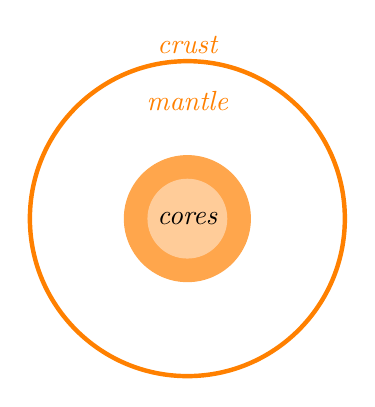
\begin{tikzpicture}

\draw[ultra thick, orange] (0, 0) circle (2cm);
\draw[orange!70,fill=orange!70](0, 0) circle (0.8);
\draw[orange!40, fill=orange!40] (0, 0) circle (0.5cm);

\pause
\node (2) at (0, 0) {\textit{\textcolor{black}{cores}}};
\node (0) at (0, 2.2) {\textit{\textcolor{orange}{crust}}};
\node (1) at (0, 1.5) {\textit{\textcolor{orange}{mantle}}};

\end{tikzpicture}
\end{document}